\subsection{Memory}\label{ssec:memory}

The memory study runs the whole package over the five libraries for $5$ rounds and $60$ seeds, with $8$ generations of $10$ crosses per round, in five arms: the full system (boosters, memory, retrieval, the committee of proposers); the full system without retrieval, which keeps the memory but does not let it steer; boosters alone; no boosters; and random pairing. Every arm without memory starts each round from the library and keeps only its synapse weights. The measured quantities are the distinct survivors after each round and the checks spent on them (Fig.~\ref{fig:memory}).

\begin{figure*}[t]
\centering
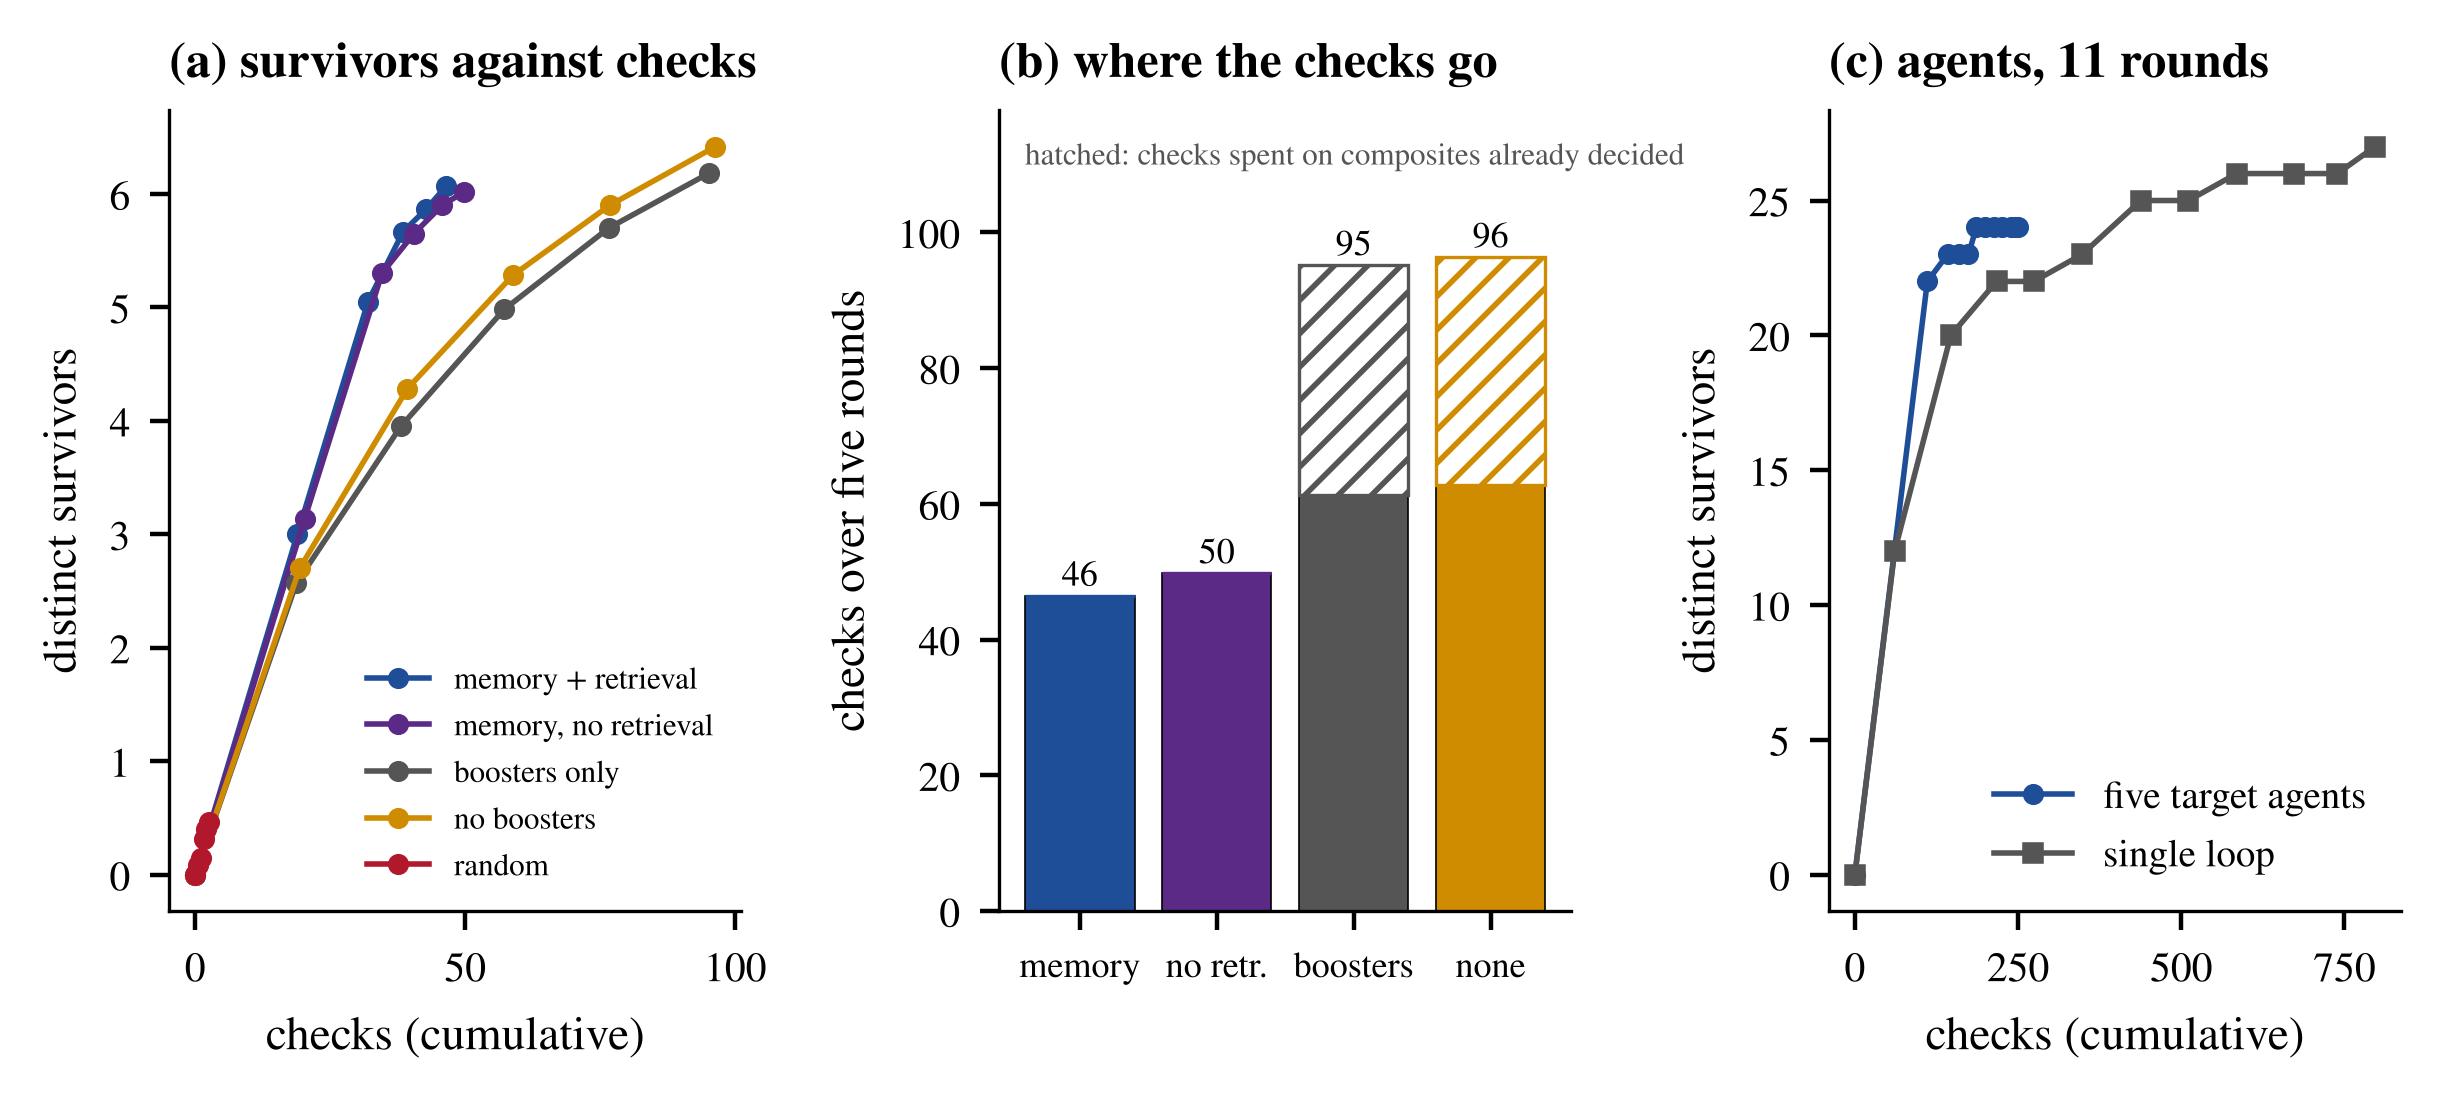
\includegraphics[width=0.98\textwidth]{figures/fig_memory}
\caption{Memory and agents. (a) Distinct survivors against cumulative checks over five rounds, mean of $60$ seeds; each marker is one round. (b) Checks over the five rounds; the hatched part is spent on composites that an earlier round of the same seed had already decided. (c) The five target agents against the single-loop control in the continuous loop, with the local model among the proposers; each marker is one round.}
\label{fig:memory}
\end{figure*}

\begin{table}[t]
\caption{The memory study: five rounds, $60$ seeds, means per seed. ``Repeated'' counts checks of composites decided in an earlier round.}
\label{tab:memory}
\centering
\footnotesize
\setlength{\tabcolsep}{3.5pt}
\begin{tabular}{@{}lrrrr@{}}
\toprule
Arm & Checks & Repeated & Survivors & Refuted \\
\midrule
full system & $46.4$ & $0.0$ & $6.07$ & $5.2$ \\
no retrieval & $49.8$ & $0.0$ & $6.02$ & $5.3$ \\
boosters only & $95.2$ & $33.9$ & $6.18$ & $10.6$ \\
no boosters & $96.3$ & $33.6$ & $6.42$ & $10.6$ \\
random & $2.5$ & $0.1$ & $0.47$ & $0.3$ \\
\bottomrule
\end{tabular}
\end{table}

Every arm except random pairing ends between $6.0$ and $6.4$ distinct survivors, because the five libraries hold that many checkable statements within reach of the crosses; all of them are known results. The arms differ in cost (Table~\ref{tab:memory}). With memory the system reaches the plateau with $46.4$ checks, against $95.2$ for boosters alone, and spends none on composites already decided; without memory a third of the checks after the first round are repeats. Retrieval steers the draw but changes little, $46.4$ checks against $49.8$: the saving comes from not checking a decided composite twice, which is the soundness bookkeeping of Section~\ref{sec:chains} applied across rounds. Memory therefore halves the cost of reaching what the libraries can reach, and it does not move the plateau.

\subsection{The channel and the agents}\label{ssec:agentsexp}

The channel study runs the five agents on one shared memory for $6$ rounds and $60$ seeds in three arms: the channel with the target weights, the target weights alone, and neither. The three arms spend $211.8$, $218.0$ and $216.8$ checks per seed over the six rounds, with standard errors below one check, and end with $24.05$, $24.15$ and $24.23$ distinct survivors. The channel saves three per cent of the checks, because a bundle that carries a failed cell halves the weight of its candidate, and it costs a tenth of a survivor for the same reason. In none of the $180$ runs does a survivor reach a target point. The channel delivers everything the engine holds, and what the engine holds are outputs of library constructions; no library holds the input that a target point needs (Section~\ref{ssec:whyhard}).

The continuous loop runs the five agents and, beside them, a single-loop control: one attack over all five libraries with boosters and no memory, $6$ generations of $40$ crosses per round. The agents use the channel, the target weights and the local model. After eleven rounds the agents hold $24$ distinct survivors for $250$ checks and the control $27$ for $797$ (Fig.~\ref{fig:memory}(c)). The agents reach $23$ survivors in the second round, for $142$ checks, and $24$ in the fifth; the control needs five rounds and $348$ checks to reach $23$ and passes the agents in the sixth round, still adding a known result every few rounds at about $70$ checks per round. No survivor of either reaches a target point. Agents are cheaper for the same reason as memory, since each agent skips what its slice of the store has decided, and they reach no further, since a target point needs an input that no library holds; the control's three extra survivors are known results that the agents' narrower libraries do not contain.

\subsection{The barrier and pattern matrix}\label{ssec:matrix}

The last experiment is done by hand and recorded in the package. For each blocking step, every pattern that broke a comparable barrier elsewhere is transferred, and the transferred statement, its needed input and the outcome are written as one cell: \emph{closes} when the pass line is crossed, \emph{partial} when a weaker statement follows or a new fact is computed, \emph{fails} when the needed input is false or unknown, with the reason. There are $38$ cells. None closes; $7$ are partial and $31$ fail. The partial cells are the forest gauge fixing and its ceiling, the box Dobrushin--Shlosman criterion as a finite check not yet run, size colourings and Theorem~\ref{thm:fvalues}, the forced arithmetic progressions in level colourings, the Kuga--Satake reduction of Varesco, the averaged Chowla theorem, and the grid search at $n=20$. The failures fall into three kinds: the input is known to be false (product colourings and m-sequence colourings for Erd\H{o}s problem 1183, plaquette variables, abelian duality for $\mathrm{SU}(2)$), the input is the open problem itself or another benchmark (motivated cycles, which are algebraic exactly when the standard conjecture holds; the inverse of $L$ as a Hodge class on $X\times X$), or the input needs a small parameter that is not small at the blocking step (Ba{\l}aban, Brydges--Yau, Kotecký--Preiss). The matrix is the content of the cells $\pi_{\mathrm{ch}}$ of \eqref{eq:channelprior} reads, so a pattern recorded as failing on a benchmark is drawn half as often there.

Two cells are new computations and one is a new negative result.

\begin{proposition}\label{prop:productrules}
Let $c_{1},c_{2}$ be level colourings of $2^{[a]}$ and $2^{[b]}$ attaining $f(a)$ and $f(b)$, and colour $S\subseteq[a+b]$ by $\phi(c_{1}(S\cap[a]),c_{2}(S\setminus[a]))$ for a Boolean function $\phi$ of two variables that depends on both. For $a=b=4$ the largest monochromatic sublattice has $16$ members when $\phi$ is exclusive or or its negation, $32$ for disjunction and $48$ for conjunction, against $f(4)+f(4)=6$.
\end{proposition}

The values are computed by the grid search of Lemma~\ref{lem:levelposet} with two blocks. They show why subadditivity $f(a+b)\le f(a)+f(b)+C$ cannot come from such products: a monochromatic sublattice of the product projects to sublattices of the factors, but the colour of a product point is a function of both factors, so the projections need not be monochromatic, and the product lattice of two chains is a grid with $(a+1)(b+1)$ members.

At $n=20$ the grid colourings with two blocks of sizes $18$ and $2$, $57$ grid points, were searched by simulated annealing on the number of pairs (colour, base point) from which a monochromatic sublattice of $12$ members is reachable. Of $24$ restarts, $16$ end with exactly one such pair and none with zero; every colouring obtained from the best one by changing one or two grid points keeps a bad pair. Refining the best colouring to three blocks of sizes $(16,2,2)$ and $(17,1,2)$ and annealing again, four restarts, also ends at one bad pair. The search does not decide $f(20)$, which remains in $\{11,12\}$.

The colourings with the shortest monochromatic progressions known come from finite fields, and they were the natural candidates for an answer to Question~9.3. They fail.

\begin{proposition}\label{prop:mseq}
Let $\alpha$ be a primitive element of $\mathbb{F}_{2^{p}}$, $\beta\neq0$, $n\le2^{p}-2$, and colour $S\subseteq[n]$ by $\mathrm{Tr}(\beta\alpha^{|S|})$. \textup{(i)} If $p$ is prime, every monochromatic sublattice isomorphic to a Boolean lattice has at most $2^{p-1}$ members. \textup{(ii)} If $\alpha^{e}=1+\alpha^{d}$ and $\mathrm{Tr}(\beta\alpha^{t+jd})=0$ for $0\le j\le k$, with $t+k\max(d,e)\le n$, there is a monochromatic sublattice with $3^{k}$ members. If $\alpha$ is a root of the trinomial $x^{p}+x+1$ and $n=2^{p}-2$, a suitable $\beta$ allows $d=1$, $e=p$, $t=0$ and $k=p-2$, which gives $3^{p-2}=\frac19(n+2)^{\log_{2}3}$ members.
\end{proposition}

\begin{proof}
A Boolean sublattice of rank $k$ is $J(P)$ for an antichain $P=\{1,\dots,k\}$ with weights $w_{i}$ and base $t$, and its members have colours $\mathrm{Tr}(\beta x)$ for $x$ in $X=\{\alpha^{t}\prod_{i\in I}\alpha^{w_{i}}\}$, whose span is $\alpha^{t}\prod_{i}\mathrm{span}\{1,\alpha^{w_{i}}\}$; each factor is a plane, since $1\le w_{i}\le2^{p}-2$. For prime $p$ the field $\mathbb{F}_{2^{p}}$ has no subfield other than $\mathbb{F}_{2}$ and itself, so the theorem of Hou, Leung and Xiang \cite{HLX02} gives $\dim(UV)\ge\min(p,\dim U+\dim V-1)$ for nonzero subspaces $U,V$, and the span has dimension at least $\min(p,k+1)$. Colour $0$ puts it in a hyperplane, so $k\le p-2$. For colour $1$ the differences $\alpha^{t}(1+\alpha^{w_{j}})\prod_{i\in I}\alpha^{w_{i}}$, $I\not\ni j$, have trace $0$ and span a product of $k-1$ planes times one element, so $k\le p-1$. This is (i). For (ii) take $k$ disjoint chains, each with ranks $0$, $d$ and $e$. Their down-sets have ranks $t+ad+be$ with $a+b\le k$, and $\alpha^{t+ad+be}=\alpha^{t}(\alpha^{d})^{a}(1+\alpha^{d})^{b}$ lies in the span of $\alpha^{t},\alpha^{t+d},\dots,\alpha^{t+kd}$, so every member has trace $0$, and $t+k\max(d,e)\le n$ keeps all ranks in range. The sublattice has $3^{k}$ members. For the trinomial, $\alpha^{p}=1+\alpha$, and the condition asks for a run of $k+1$ zeros in the $m$-sequence $\mathrm{Tr}(\beta\alpha^{i})$; each period has a run of $p-1$ zeros, choosing $\beta$ moves it to $t=0$, and $(p-2)p\le2^{p}-2$.
\end{proof}

For the colourings defined by $x^{5}+x^{2}+1$, $x^{6}+x+1$ and $x^{7}+x+1$ at $n=2^{p}-2$, the largest sublattices of the form (ii) have $27$, $81$ and $243$ members, or $0.84$, $1.27$ and $1.90$ times $n+2$, with $(d,e)=(2,5)$, $(1,6)$ and $(1,7)$. The linearity that keeps the progressions of both classes at length $p-1$ turns every progression whose difference has a small partner $e$ into a triangle of ranks, so an answer to Question~9.3 by level colourings needs classes that avoid both.
